\documentclass[11pt,letter]{exam}
\usepackage{listings}

\newif\ifpdf
\ifx\pdfoutput\undefined
\pdffalse % we are not running PDFLaTeX
\else
\pdfoutput=1 % we are running PDFLaTeX
\pdftrue
\fi

\ifpdf
\usepackage{subfigure}
\usepackage[pdftex]{graphicx}
\else
\usepackage{graphicx}
\fi

\firstpageheader{\bf\Large CS 151}{\bf\Large Exam-2}{\bf\Large
  April 8, 2004}
\runningheader{CS 151}{}{Exam-2}
\addpoints

\begin{document}
\begin{center} 
  \fbox{\fbox{\parbox{5.5in}{\centering This Quiz is being given under
        the guidelines of the \textbf{Honor Code}. You are expected to
        respect those guidelines and to report those who do not.
        Answer the questions in the spaces provided. If you run out of
        room for an answer, continue on the back of the page.  There are
      \numquestions\  questions for a total of  \numpoints\ points.}}}
\end{center} 
\lstset{language=Java,numbers=left}

\vspace{0.1in} 
\hbox to \textwidth{Name:\enspace\hrulefill} 


\begin{questions}

\question[5] What is the running time for the following algorithm?
\vspace{0.5in}

\begin{lstlisting}
public static boolean isPrime( int n ) {
   if( n == 2 || n == 3 )
      return true;
   if( n % 2 == 0 )
     return false; 
   for( int i = 3; i <= squareRoot( n ); i+=2 )
     if( n % i == 0 )
        return false; 
   return true; 
}
\end{lstlisting}

% Write a recursive function
\question[15] Replace the loop in lines 6-9 with a recursive helper
function.  \textit{Hint:} The helper should take two parameters.

\vspace{5in}

% Trace the operation of this 
\question Given the following recursive function:
\begin{lstlisting}
private void mystery( char [ ] str, int low, int high )     {
   if( low < high )
       println( str );
   for( int i = low; i <= high; i++ )         {
       char [ ] tmp = str.clone( ); // tmp will be str
       tmp[ i ]   = str[ low ];     // with i and low
       tmp[ low ] = str[ i ];       // swapped
       mystery( tmp, low + 1, high );
   }     
} 
\end{lstlisting}
\begin{parts}
  \part[20] Trace the calls for mystery when it is called as follows:
  \texttt{mystery("abc", 0, 2);}
\vspace{6in}
\part[5] what is the running time for mystery in big O terms?
\vspace{.5in}
\part (5 points \textbf{extra credit}) Rewrite mystery so it is not recursive.

\end{parts}


% remove duplicates from a list
\newpage
\question[20] 
  Write an 
  $O(n \log{n})$ algorithm that will remove all duplicates from an
  array of $n$ floats.  You may use Arrays.sort(), but no other Classes
  from the Java Collections library.
\vspace{4.5in}

\newpage
\question[10] Using the \textit{Median of 3} approach, show how
quicksort would parition the following array of numbers.  When you are
done make sure that you clearly identify $L$, $R$, and the pivot.
\begin{figure}[h]
  \centering
  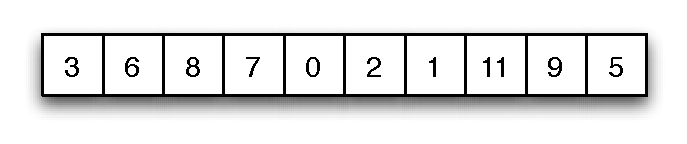
\includegraphics{part-array.pdf}
\end{figure}

\newpage \question[10] Given the following array $int[] a = \{ 90, 1,
3, 8, 56, 21, 5, 13, 1, 146, 2, 34\}$.  Show the contents of $a$
during shell sort, after a gap size of 5, 2, and 1.  \textbf{Note
  Bene} You do not need to show every swap, just the contents after
the processing for each gap size.


\end{questions}

\end{document}


% Local Variables:
% mode: LaTeX
% mode: Auto-Fill
% mode: RefTeX
% mode: Flyspell
% End:
